\subsection{Drivetrain}\label{Drivetrain}

%% INTRODUCTION %%
The drive train on the given belt vehicle is what translates the torque $\tau_m$ given by the motor into the actual movement of the vehicle. The model of this system part shows the relation between the applied rotational force (or torque) $\tau_m$ and the speed of the belts. It is still considered that the vehicle's tajectory follows a straight line.\\\\
%
Different iterations of this model can be made to get more acuraccy. The first of these iterations should give an overview of how the system reacts to a given torque input. 

%% SSSECTION : BLACK BOX MODEL %%
\subsubsection{Black Box Model}\label{BlackBoxModel}
To get a rough approximation of how the drive train works, a black box model is used. There is a small gear $G_m$ on the motor shaft, which is in contact with another actual gear $G_2$. The imaginary gear $G_d$ represents the differential and the gears and shafts of the drivetrain from (and including) this second gear $G_2$ to the gears that drive the belt, see \figref{fig:DrivetrainMechanicalModel} and \figref{fig:BeltMechanicalDiagram}.

\begin{figure}[H]
	\centering
	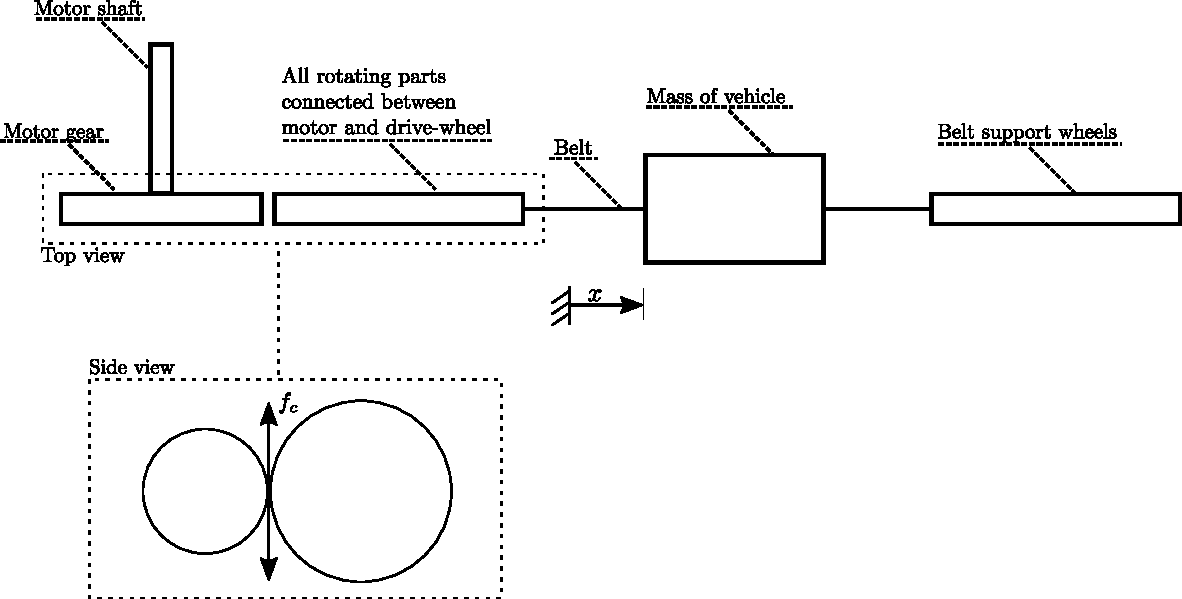
\includegraphics[scale=0.8]{figures/mechanicalDrawing.pdf}
	\caption{A simple mechanical diagram of the vehicle drivetrain}
	\label{fig:DrivetrainMechanicalModel}
\end{figure}
\todo{Add notations to the diagram and create free body diagrams of belt and black box parts}

%% DEFINITION OF NEWTON'S PRINCIPLE %%
Newton's second law is the main formula to use for mechanical models of a system. It can be written as :

\begin{flalign}\centering
M \cdot a = \sum F_{ext}
\label{eq:mechanicalmodel}
\end{flalign}
\hspace{6mm} Where\\
\begin{tabular}{p{1cm}ll}
& $M$							& is the system's mass [$kg \cdot m^2$] \\
& $a = \dot v$ 		& is the linear acceleration of the system [$m \cdot s^{-2}$] \\
& $v$ 						& is the linear velocity of the system [$m \cdot s^{-1}$] \\
& $\sum F_{ext}$	& is the sum of external forces applied to the system [$N$] \\
\end{tabular},

which can also be applied to rotational systems as :

\begin{flalign}\centering
J \cdot \alpha = \sum \tau_{ext}
\label{eq:mechanicalmodel}
\end{flalign}
\hspace{6mm} Where\\
\begin{tabular}{p{1cm}ll}
& $J$											& is the system's inertia [$kg \cdot m^2$] \\
& $\alpha = \dot{\omega}$ & is the rotational acceleration of the system [$m \cdot s^{-2}$] \\
& $\omega$ 								& is the rotational velocity of the system [$m \cdot s^{-1}$] \\
& $\sum \tau_{ext}$  			& is the sum of external torques applied to the system [$N \cdot m$] \\
\end{tabular}.

%% APPLICATION OF NEWTON'S SECOND LAW %%

\begin{figure}[H]
	\centering
	%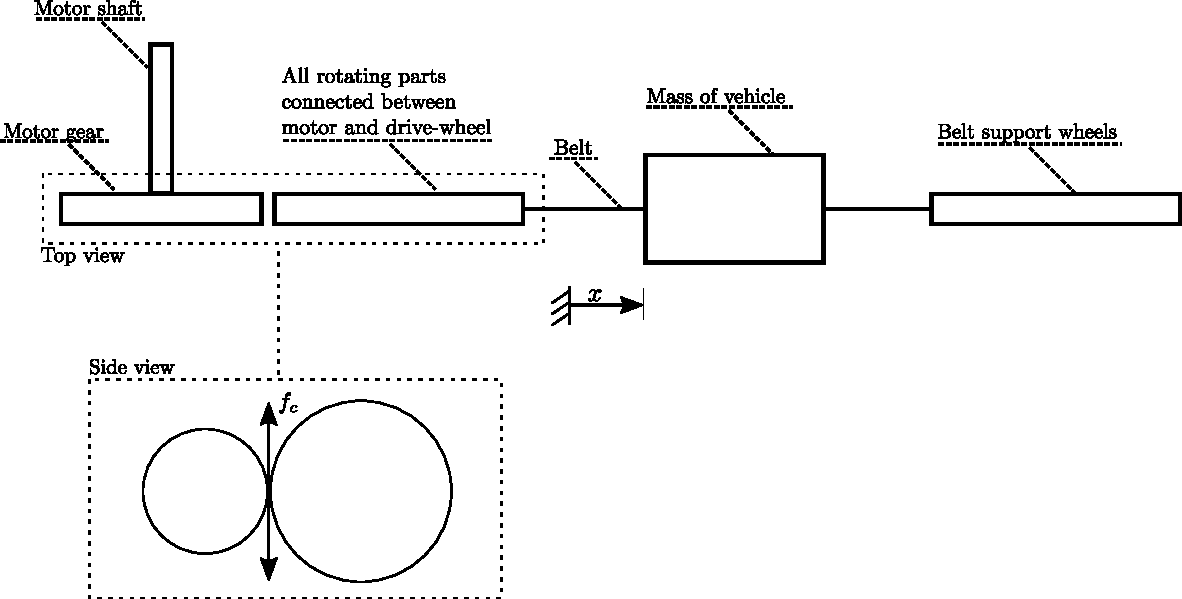
\includegraphics[scale=0.8]{figures/mechanicalDrawing.pdf}
	\caption{A free body diagram of the motor gear}
	\label{fig:MotorGearFreeBodyDiagram}
\end{figure}

\begin{figure}[H]
	\centering
	%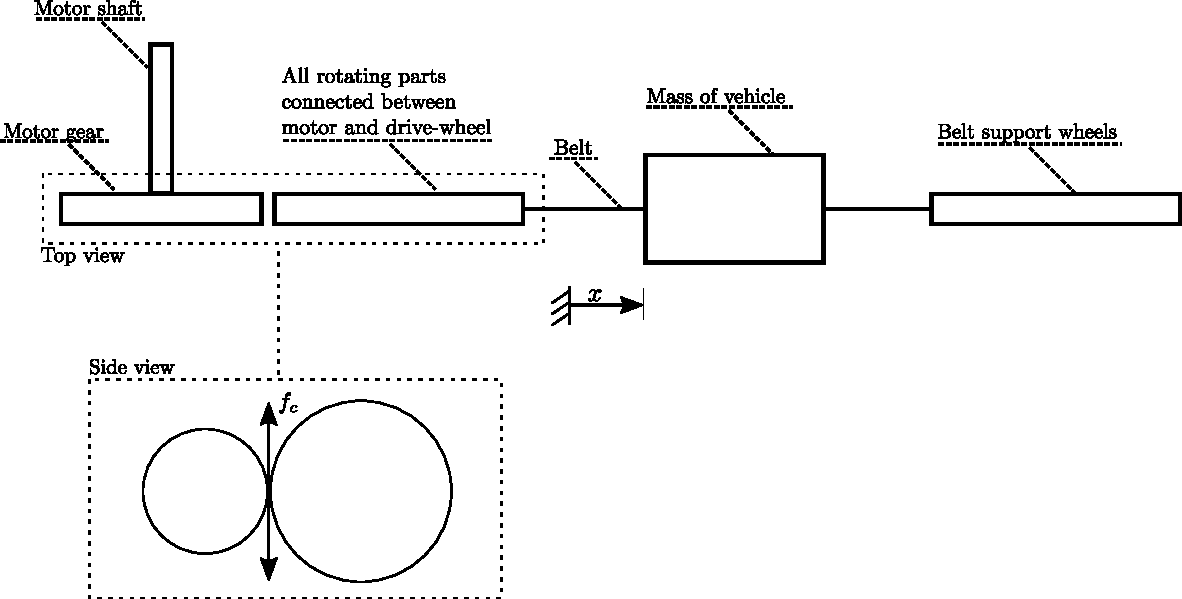
\includegraphics[scale=0.8]{figures/mechanicalDrawing.pdf}
	\caption{A free body diagram of the `black-box' gear}
	\label{fig:BlackBoxGearFreeBodyDiagram}
\end{figure}

From \figref{fig:MotorGearFreeBodyDiagram} and Newton's second law appplied to rotational systems, the following equation can be extracted:

\begin{flalign}\centering
J_m \cdot \dot{\omega}_m(t) = \tau_m(t) - B_m \cdot \omega_m(t) - N_m \cdot f_c(t) 
\label{eq:mechanicalmodel}
\end{flalign}
\hspace{6mm} Where\\
\begin{tabular}{p{1cm}ll}
& $J_m$ 			      & is the motor's inertia [$kg \cdot m^2$] \\
& $\omega_m$        & is the angular velocity of the motor [$rad \cdot s^{-1}$] \\
& $\dot{\omega}_m$ 	& is the angular acceleration of the motor [$rad \cdot s^{-2}$] \\
& $\tau_m$ 		     	& is the torque delivered by the motor [$N \cdot m$] \\
& $B_m$             & is the coefficient of the friction happening inside the motor [$N \cdot s \cdot rad^{-1}$] \\
& $N_m$             & is the number of teeth of the motor gear $G_m$ [$number\ of\ teeths$] \\
& $f_c$             & is the coefficient of the contact force between $G_m$ and $G_d$ [$N \cdot number\ of\ teeths^{-1}$]
\end{tabular}
\todo{Discuss about units (use siunitx?) and equations conventions inside the report}

The equation for \figref{fig:BlackBoxGearFreeBodyDiagram} is obtained the same way:

\begin{flalign}\centering
J_d \cdot \dot{\omega}_d(t) = N_d \cdot f_c(t) - N_d \cdot f_b
\label{eq:mechanicalmodel}
\end{flalign}
\hspace{6mm} Where\\
\begin{tabular}{p{1cm}ll}
& $J_m$ 			      & is the motor's inertia [$kg \cdot m^2$] \\
& $\omega_m$        & is the angular velocity of the motor [$rad \cdot s^{-1}$] \\
& $\dot{\omega}_m$ 	& is the angular acceleration of the motor [$rad \cdot s^{-2}$] \\
& $N_d$ 		     		& is the torque delivered by the motor [$N \cdot m$] \\
& $f_c$             & is the coefficient of the contact force between $G_m$ and $G_d$ [$N \cdot number\ of\ teeths^{-1}$] \\
& $f_b$             & is the coefficient of the contact force between $G_d$ and the belt [$N \cdot number\ of\ teeths^{-1}$] \\
\end{tabular}

\begin{figure}[H]
	\centering
	%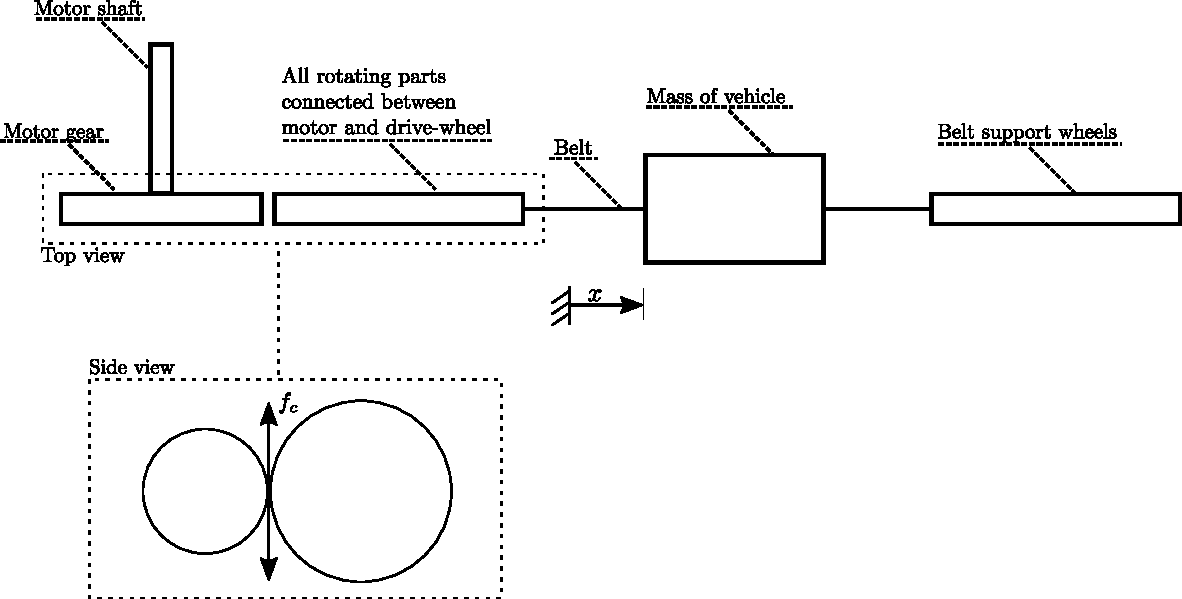
\includegraphics[scale=0.8]{figures/mechanicalDrawing.pdf}
	\caption{A mechanical diagram of the belt part}
	\label{fig:BeltMechanicalDiagram}
\end{figure}

\begin{figure}[H]
	\centering
	%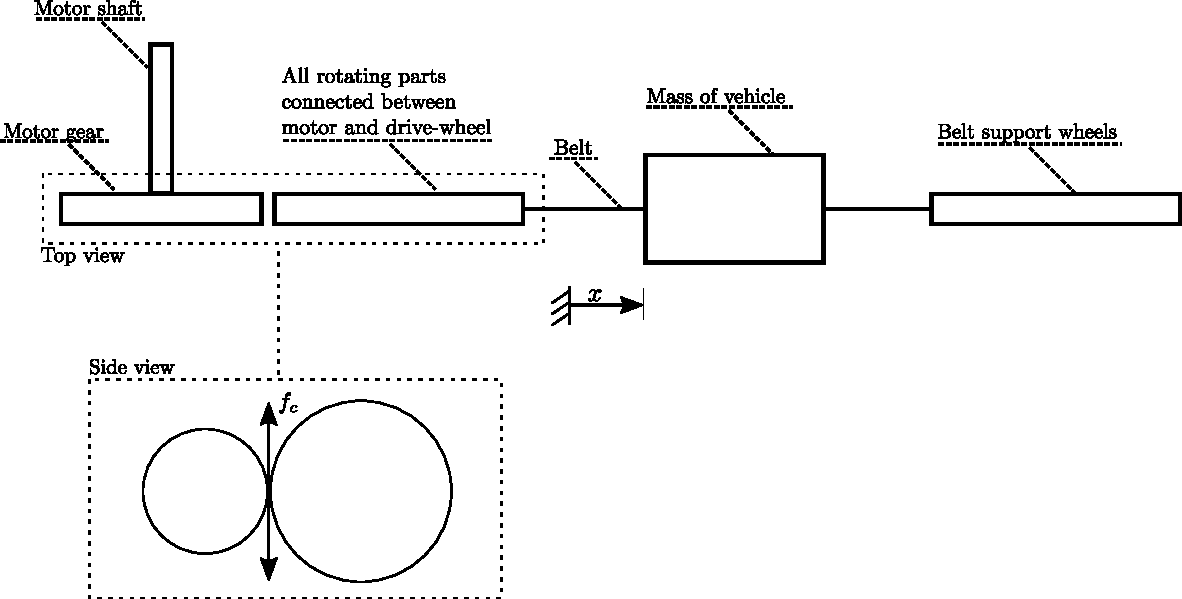
\includegraphics[scale=0.8]{figures/mechanicalDrawing.pdf}
	\caption{A free body diagram of the belt driven mass}
	\label{fig:BeltFreeBodyDiagram}
\end{figure}

And eventually, the mechanical equation of the belt system on \figref{fig:BeltFreeBodyDiagram} is :

\begin{flalign}\centering
M \cdot \dot{v}(t) = r_t \cdot f_b - B_{sys} \cdot v
\label{eq:mechanicalmodel}
\end{flalign}
\hspace{6mm} Where\\
\begin{tabular}{p{1cm}ll}
& $M$ 			  & is the vehicle's total weight [$kg$] \\
& $v$        	& is the linear velocity of the behicle [$m \cdot s^{-1}$] \\
& $\dot{v}$ 	& is the linear acceleration of the vehicle [$m \cdot s^{-2}$] \\
& $r_t$ 		  & is the translational coefficient between the last gear and the belt [$m \cdot number\ of\ teeths^{-1}$] \\
& $B_{sys}$   & is the coefficient of the friction happening throughout the gears [$N \cdot s \cdot rad^{-1}$] \\
\end{tabular}